\section{Descrizione del progetto}
Per quanto riguarda la parte di ASM  \textit{ASM} si è deciso di riprendere un esempio visto in classe (e durante le pause), ovvero quello relativo alla \textit{\textbf{Coffee machine}}.
Il distributore modellato può preparare diversi tipi di bevande (caffè, cappuccino etc), ognuna preparata con diverse quantità di ingredienti (acqua, caffè, latte etc) i quali vengono consumati e devono essere reintegrati dal manutentore.	

Il distributore accetta pagamenti solamente in moneta tramite l'inserimento di denaro nell'apposita fessura.

Il distributore è in grado di fornire il resto (anche se non sempre in modo esatto).

Quando tutte le bevande sono esaurite, il distributore va fuori servizio, in attesa che gli ingredienti vengano aggiunti dal manutentore, il quale può inoltre prelevare o inserire monete dal distributore, sempr etenendo conto del vincolo di capacità del vano porta monete.

\section{Macchina a stati}
La ASM è basata su una sottostante macchina a stati finiti, mostrata in figura, che definisce i principali stati e transizioni del distributore. La ASM permette di estendere questa FSM introducendo un concetto aumentato di “stato”, che comprende anche funzioni dinamiche, modificando le quali si possono memorizzare informazioni aggiuntive.

\begin{figure}[h]
	\centering
	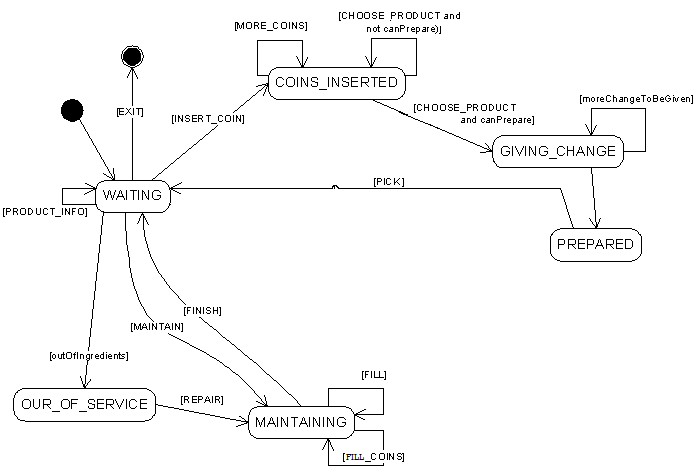
\includegraphics[width=0.8\textwidth]{Immagini/FSM.png}
	\caption{Macchina a stati}
	\label{fig:StateMachine}
\end{figure}

In particolare, è stato possibile memorizzare informazioni su:
\begin{itemize}
	\item Quantità di ingredienti residui
	\item Monete possedute dal distributore
	\item Credito dell'utente attuale
\end{itemize}

\section{Standard Library}



